\subsection{Implementierung mit React}
%\subsubsection{Vorstellung des Frameworks}
Zur Erstellung des Front-Ends der Webanwendung werden hauptsächlich die etablierten Technologien \ac{HTML}, \ac{CSS} und JavaScript benutzt.

Zusätzlich wird React, eine JavaScript-Bibliothek, verwendet.
React\footnote{\url{https://reactjs.org}} ist ein Framework, welches seit 2013 von Facebook als Open-Source-Lösung bereitgestellt wird.\autocite[Vgl.][S. 3]{React2019} 

Eine weitere beliebte Option zur Erstellung von interaktiven Webanwendungen ist Angular\footnote{\url{https://angular.io}}. In dem vorliegenden Projekt wurde entschieden React zu verwenden, da die Technologie als Einsteigerfreundlicher als Angular eingeschätzt wurde und sich somit für das kolloborative Entwickeln in dem großen Projektteam sehr gut eignet. Darüber hinaus lässt sich der Entwurf in Kapitel \vref{ch:Entwurf} mit React gut umsetzen.

Mit React können effizient sogenannte \ac{SPA} entwickelt werden. 
Eine \ac{SPA} ist eine Webanwendung, die aus lediglich einer \ac{HTML}-Seite besteht und deren Inhalte dynamisch zur Laufzeit nachgeladen bzw. erweitert werden.
Der Kern von React liegt auf einem komponentenbasierten Aufbau der Webanwendungen sowie der jeweiligen Anordnung der Komponenten.\autocite[Vgl.][S. 3]{React2019} 

Komponenten sind unabhängige, wiederverwendbare Entitäten, die durch eine hierarchische Komposition die Inhalte der \ac{SPA} bestimmen und beliebig tief verschachtelt werden können.
In React werden zwei Typen von Komponenten unterschieden. 
Zum einen können funktionale Komponenten erzeugt werden, die JavaScript-Funktionen umfassen. 
Zum anderen werden klassenbasierte Komponenten verwendet. 
Diese sind JavaScript-Klassen, die eine höhere Komplexität aufweisen, jedoch auch mehr Funktionalitäten besitzen. 

Darüber hinaus sind in React insbesondere die Konzepte \textit{Properties}, zu Deutsch Eigenschaften, und der \textit{State}, zu Deutsch Zustand. 
Mithilfe von \textit{Properties} können Komponenten Informationen austauschen, sodass beispielsweise eine Eltern-Komponente relevante Informationen an eine Kind-Komponente weitergibt. 
Die übergebenen Werte der Properties können jedoch nicht geändert werden. 

Dementgegen können sich die Werte bei dem Konzept \textit{State} ändern. 
Zu jeder Komponente gibt es einen Objekt-Zustand, \texttt{this.state}, worauf nur die Komponente selbst zugreifen und den Wert ändern kann. 
Der State einer Komponente enthält Eigenschaften, die von der Komponente beobachtet werden können. 
Wenn sich der State einer Komponente ändert, wird der \ac{DOM} angepasst und die Komponente mit den aktualisierten Werten gerendert. 

Sobald Änderungen den Inhalt der Webanwendung verändern, wird bei React nicht der komplette Seiteninhalt angepasst, sondern lediglich die tatsächliche Veränderungen bei dem entsprechenden \ac{DOM}-Element vorgenommen. 
Der Vorteil hierbei ist, dass die Benutzeroberfläche schneller auf Veränderungen reagieren kann. 

\textit{Todo (Entwicklung derzeit in Progress)}
\begin{itemize}
	\item Ordnerstruktur in Abbildung \vref{fig:Front-End_Ordnerstruktur}
	\item Aufbau einer Hauptkomponente, JSX erklären
	\item UI Gestaltung mit Material-UI (https://material-ui.com/):
		\subitem Grund: bietet viele nützliche UI Komponenten und Design System für React -> vereinfacht Entwicklung
	\item Dynamische Seitenverwaltung: Virtuelles \ac{DOM}
	\item React-Routing: über Proxy in Dev; in Prod ohne
\end{itemize}

\begin{figure}[H]
	\centering 
	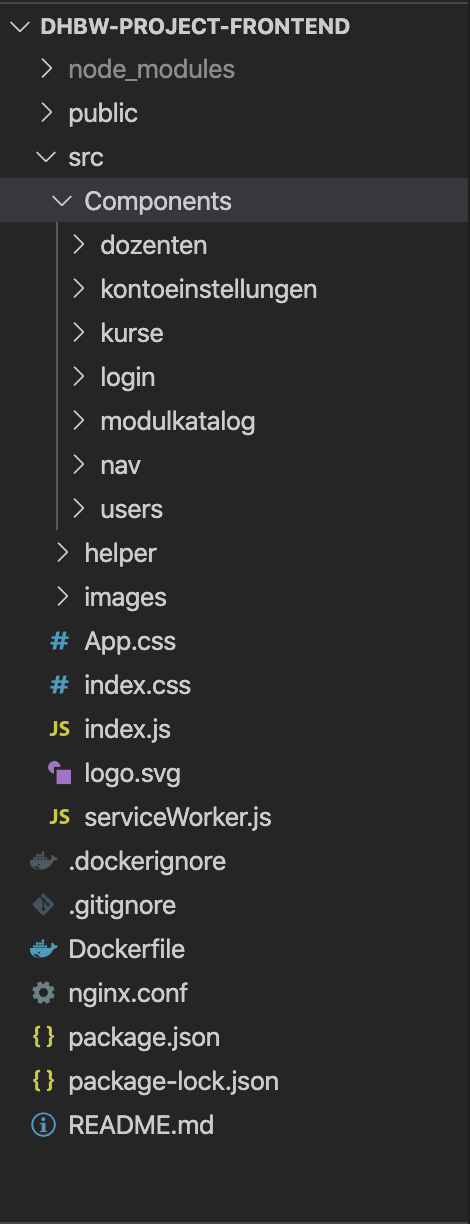
\includegraphics[scale=0.75]{img/FrontEnd/front-end-ordnerstruktur}
	\caption[Übersicht der Ordnerstruktur des Front-Ends]{\label{fig:Front-End_Ordnerstruktur}Übersicht der Ordnerstruktur des Front-Ends\footnotemark}
\end{figure}
\footnotetext{Verwendete Entwicklungsumgebung: Visual Studio Code (\url{https://code.visualstudio.com})}

